\documentclass{beamer}
\setbeamertemplate{footline}[frame number]
\usetheme{Ilmenau}
\usecolortheme{dove}
\usepackage{amsmath}
\usepackage{amssymb}
\usepackage{wasysym}
\usepackage{commath}
\usepackage{xcolor}
\definecolor{oxblue}{RGB}{0, 0, 51}
\usepackage{graphicx}
\usepackage{tikz}
\usetikzlibrary{calc}
\usepackage{tkz-euclide}
\usepackage{caption}
\usepackage{subcaption}
\usepackage{float}
\mode<presentation>{}
\usepackage[backend=biber, citestyle=authoryear]{biblatex}
\addbibresource{pres.bib}

\setbeameroption{show notes}

\title{\color{oxblue}{\sc{Stripped Down Cluster Galaxies with Gravitational Lensing}}}
\subtitle{\sc{Part III Presentation}}
\author{\sc{Joe Winterburn}}
\institute{\sc{Institute of Astronomy}}
\date{}



\begin{document}

  \begin{frame}
    \titlepage
  \end{frame}

  \begin{frame}
    \frametitle{\sc Outline}
    \tableofcontents
  \end{frame}

  \section{Background}

  \subsection{Motivations}

  \begin{frame}
    \frametitle{Motivations}
    \begin{itemize}
      \item Lensing directly measures fractional energy density of matter.
      \note{Lensing is a useful probe for $\Omega_m$ in the universe.\\}
      \item Lensing statistics can be used to probe properties of galaxy populations.
      \note{Quantities (convergence, shear, magnification) and statistics (correlation functions, galaxy-galaxy signal) can be computed for galaxy populations.\\}
      \item The effects of tidal stripping in satelite vs central populations can be explored.
      \note{Correlation functions can show differences between these two galaxy populations, and these can be eput into context of the galactic halo model.\\}
      \item Lensing doesn't rely on assumptions about dynamical environment or dark matter distribution.
      \note{Makes it a very useful probe for imaging surveys.\\}
      \item Computing lensing statistics in hydrodynamical simulations and comparing to observation allows constraints to be put on models.
      \note{Some research has been done on this recently, more on that to come.\\}
    \end{itemize}
  \end{frame}

  \begin{frame}
    \begin{itemize}
      \item (\cite{bah2021}) recently explored the claim that cluster subhaloes are more abundant than $\Lambda$CDM predictions.
      \item (\cite{M20}) highlighted this issue and proposed that either there are systematic issues with simulations or incorrect assumptions about dark matter.
      \item (\cite{bah2021}) concludes that there is no tension with $\Lambda$CDM models, but the observed abundances can provide constraints on baryonic physics in simulations.
      \item The take-away is that one needs to be careful about limiting resolution on small scales in cosmological simulations.
    \end{itemize}
  \end{frame}

  \subsection{Horizon AGN}

  \begin{frame}
    \frametitle{\sc Horizon AGN}
    The data made available to me is from the Horizon AGN simulation:
    \begin{itemize}
      \item Cosmological hydrodynamical simulation performed with RAMSES.
      \item $1024^3$ dark matter particles.
      \item Mass resolution of $8\times 10^7 h^{-1} \text{M}_{\astrosun}$.
      \item Lensing quantities (deflection) generated by multiple lens-plane raytracing through the lightcone.
      \note{I believe the raytracing was performed at each simulation time step during the dynamical simulation.\\}
      \item Field of view: 1 deg$^2$ up to $z\approx 7$, 2.25 deg$^2$ up to $z\approx 1$.
      \note{The deep lightcone deflection map is a product of considering 500 transverse lens planes with varying comoving thickness.}
    \end{itemize}
  \end{frame}

  \begin{frame}
    
  \end{frame}

  \subsection{Gravitational Lensing}

  \begin{frame}
    \frametitle{\sc Gravitational Lensing}
    Einstein's General Relativity predicts the gravitational deflection of photons by mass distributions, famously confirmed experimentally by Eddington in 1919.
    \\
    \centering
    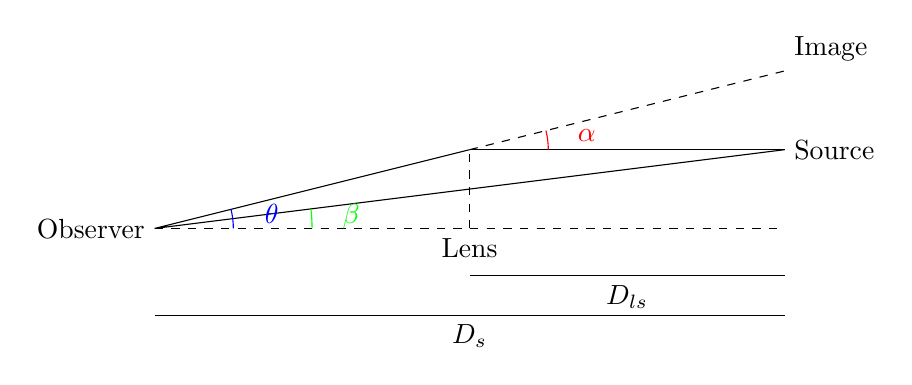
\begin{tikzpicture}
      \coordinate (A) at (-4, 0);
      \coordinate (B) at (0, 0);
      \coordinate (C) at (4, 0);
      \coordinate (D) at (4, 1);
      \coordinate (E) at (4, 2);
      \coordinate (F) at (0,1);

      \draw[thin, black] (F)--(A)--(D);
      \draw[thin, black, dashed] (F)--(E);
      \draw[thin, black] (F)--(D);
      \draw[thin, black, dashed] (B)--(F);
      \draw[thin, black, dashed] (A)--(C);

      \draw (A) node[left] {Observer};
      \draw (B) node[below] {Lens};
      \draw (D) node[right] {Source};
      \draw (E) node[above right] {Image};

      \draw[thin, black] (0, -0.6) -- (4, -0.6) node[midway, below] {$D_{ls}$};

      \draw[thin, black] (-4, -1.1) -- (4, -1.1) node[midway, below] {$D_s$};

      \tkzMarkAngle[blue, opacity=1, size=1](B,A,F);
      \tkzLabelAngle[pos=1.5](B,A,F){$\color{blue}{\theta}$};

      \tkzMarkAngle[red, opacity=1, size=1](D,F,E);
      \tkzLabelAngle[pos=1.5](D,F,E){$\color{red}{\alpha}$};

      \tkzMarkAngle[green, opacity=1, size=2](B,A,D);
      \tkzLabelAngle[pos=2.5](B,A,D){$\color{green}{\beta}$};
    \end{tikzpicture}
  \end{frame}

  \subsection{Weak Lensing}

  \begin{frame}
    The thin lens approximation gives the following relationship between the unobservable true source position $\color{green}{\vec{\beta}}$ and the observed image position $\color{blue}{\vec{\theta}}$:
    \begin{equation} \label{eq:lens}
      \color{green}{\vec{\beta}} \color{black}= \color{blue}{\vec{\theta}} - \color{black}{\frac{D_{\text{ls}}}{D_{\text{s}}}}\color{red}{\vec{\alpha}}\left( \vec{\theta} \right)\color{black}
    \end{equation}
    where the deflection angle $\color{red}{\vec{\alpha}}$ is found by integrating the gravitational potential along the line of sight. The raytracing through the lightcone discretizes the space into transverse planes, and the deflection is calculated recursively from the observer out to a given source redshift.
  \end{frame}

  \begin{frame}
    The result is a deflection map describing the two orthogonal components of $\vec{\alpha}$ at each point in the field of view. A Taylor expansion of the lens equation \ref{eq:lens} gives the Jacobian of the $\vec{\theta} \rightarrow \vec{\beta}$ mapping, defining the magnification tensor

    \begin{equation} \label{eq:mu tensor}
      a_{ij}\left( \vec{\theta} \right) = \frac{\partial\vec{\beta}}{\partial\vec{\theta}} = \delta_{ij} - \phi_{,ij} \equiv
      \begin{pmatrix}
        1 - \kappa - \gamma_1 & -\gamma_2 \\
        -\gamma_2 & 1 - \kappa + \gamma_1
      \end{pmatrix}
    \end{equation}

    with $\phi$ the lensing potential, related to the convergence $\kappa$ by $\Delta \phi = \nabla \cdot \vec{\alpha} \equiv 2\kappa$, and $\gamma_{1/2}$ the components of the spin-2 shear.
  \end{frame}

  \begin{frame}
    Hence given a deflection field defined on the field of view of a slice of the lightcone, the lensing observables can be calculated by
    \begin{align} \label{eq:lensing observables}
      \kappa &= \frac{1}{2}\left( \alpha_{1,1} + \alpha_{2,2} \right) \\
      \gamma_1 &= \frac{1}{2}\left( \alpha_{1,1} - \alpha_{2,2} \right) \\
      \gamma_2 &= \alpha_{1,2} = \alpha_{2,1}
    \end{align}
    which can be computed numerically using finite differences, yielding a convergence and shear map defined over the field of view.
  \end{frame}

  \begin{frame}
    The convergence is the projected surface mass density in the lens plane expressed in units of the critical density:
    \begin{equation} \label{eq:sigma_kappa}
      \Sigma_{\text{crit}} \kappa\left( \theta \right) = \Sigma\left( \theta \right) = \int\rho\left( \theta, z \right) \dif z.
    \end{equation}

    where the critical density is defined by

    \begin{equation} \label{eq:critical density}
      \Sigma_{\text{crit}} = \frac{c^2}{4\pi G}\frac{D_{s}}{D_{l}D_{ls}}.
    \end{equation}
  \end{frame}

  \begin{frame}
    From (\cite{agn}), the tangential shear, convergence and mean convergence enclosed inside a radius $R$ around a lensing galaxy/halo are related by

    \begin{equation} \label{eq:mean kappa}
      \bar{\kappa}\left( <R \right) = \frac{2}{R^2} \int_0^R \kappa \left( R' \right)R'\dif R' = \kappa \left( R \right) + \gamma \left( R \right).
    \end{equation}

    Using the definition of $\Sigma_{crit}$ in equation \ref{eq:critical density}, the excess density $\Delta\Sigma$ can be defined as

    \begin{equation} \label{eq:delta sigma}
      \Delta\Sigma\left( R \right) = \frac{M\left( <R \right)}{\pi R^2} - \Sigma\left( R \right) = \Sigma_{\text{crit}}\gamma\left( R \right).
    \end{equation}

    So correlation functions can be computed around a selection of lensing galaxies and the statistics can be reated to $\Sigma$ and $\Delta\Sigma$, exploring how the lensing signal differs for galaxies with differing properties.
  \end{frame}

  \subsection{Strong Lensing}

  \begin{frame}
    In the strong lensing regime, multiple images can be produced from a single source:
    \\
    \centering
    \begin{tikzpicture}
      \coordinate (A) at (-4, 0);
      \coordinate (B) at (0, 0);
      \coordinate (C) at (4, 0);
      \coordinate (D) at (0, 1);
      \coordinate (E) at (0, -1);
      \coordinate (F) at (4, 2);
      \coordinate (G) at (4, -2);

      \filldraw[oxblue] (A) circle (1pt) node[left] {Observer};
      \filldraw[oxblue] (E) circle (1pt) node[below] {Lens};
      \filldraw[oxblue] (C) circle (1pt) node[right] {Source};
      \filldraw[oxblue] (F) circle (1pt) node[right] {Image 1};
      \filldraw[oxblue] (G) circle (1pt) node[right] {Image 2};

      \draw[thin, black, dashed] (A)--(C);
      \draw[thin, black] (A)--(D);
      \draw[thin, black] (A)--(E);
      \draw[thin, black] (D)--(C);
      \draw[thin, black] (E)--(C);
      \draw[thin, black, dotted] (E)--(D);
      \draw[thin, black, dashed] (D)--(F);
      \draw[thin, black, dashed] (E)--(G);
    \end{tikzpicture}
    \\
    \raggedright
    This occurs when light rays pass through a region in which the lensing potential is sufficiently strong.
  \end{frame}

  \begin{frame}
    In this regime, the mapping $\beta \rightarrow \theta$ is no longer bijective. Given a deflection map in the image plane, for each position $\theta$ the corresponding source plane position $\beta$ can be calculated. Multiple image plane positions $\theta$ will map to the same source plane position $\beta$, defining caustic regions in the source plane from which multiple images are produced.
    \\
    From this, properties such as the optical depth for strong lensing can be calculated, and lensing galaxies/galaxy clusters can be matched to caustic regions in the source plane, allowing the opportunity to explore the effect of galaxy properties (halo environment, stellar mass etc) on the strong lensing signal.
  \end{frame}

  \subsection{Limitations}

  \begin{frame}
    \frametitle{\sc Limitations}
    A relevant limitation that comes with the simulated data available is that for larger source redshifts, there is more matter along the line of sight that contributes to the overall deflection. This makes it difficult to isolate the lensing signal due to individual objects as the source redshift increases. For this reason, analysis of correlation functions in the weak lensing regime for high redshift sources must be made cautiously.
    \\
    Another limitation is that isolating lensing galaxies at a range of redshifts from observer to source means the distances involved will vary. The overall lensing efficiency is dependent on these distances and so will vary when considering different objects in a given catalog.
  \end{frame}



  \section{Computation and Results}

  \subsection{Weak Lensing: Convergence and Shear}

  \begin{frame}
    \frametitle{\sc Convergence and Shear Maps}
    Convergence and tangential shear maps were computed from the Jacobian of the deflection fields for source redshifts $z_s = 0.39, 1.5, 4.89$ for the narrow 1 deg$^2$ field of view, and $z_s = 0.97$ for the wider 2.25 deg$^2$ field, using finite differences. The resulting maps for the largest redshift in the narrow field, and the wide field are shown:
  \end{frame}

  \begin{frame}
    \begin{figure}[H]
      \centering
      \begin{subfigure}{0.49\textwidth}
        \includegraphics[width=\textwidth]{figures/maps/kappa/kappa_0473.png}
      \end{subfigure}
      \hfill
      \begin{subfigure}{0.49\textwidth}
        \includegraphics[width=\textwidth]{figures/maps/gamma/rebin_gamma_0473.png}
      \end{subfigure}
      \hfill
      \caption{Convergence and tangential shear for $z_s = 4.89$}
      \label{fig:0473 kappa gamma}
    \end{figure}
  \end{frame}

  \begin{frame}
    \begin{figure}[H]
      \centering
      \begin{subfigure}{0.49\textwidth}
        \includegraphics[width=\textwidth]{figures/maps/kappa/kappa_0244.png}
      \end{subfigure}
      \hfill
      \begin{subfigure}{0.49\textwidth}
        \includegraphics[width=\textwidth]{figures/maps/gamma/rebin_gamma_0244.png}
      \end{subfigure}
      \hfill
      \caption{Convergence and tangential shear for $z_s = 0.97$}
      \label{fig:0244 kappa gamma}
    \end{figure}
  \end{frame}

  \begin{frame}
    As the convergence corresponds to the lensing mass distribution, it is instructive to compare the convergence profiles with the simulated light distribution from the simulation:

    \begin{figure}[H]
      \begin{subfigure}{0.49\textwidth}
        \includegraphics[width=\textwidth]{figures/maps/kappa/kappa_0473.png}
      \end{subfigure}
      \hfill
      \begin{subfigure}{0.35\textwidth}
        \includegraphics[width=\textwidth]{figures/hagn/HAGN_img.png}
      \end{subfigure}
      \hfill
    \end{figure}

    A clear correspondence with the convergence map and light distribution can be seen.
  \end{frame}

  \begin{frame}
    Zooming into the main cluster, one can compare the tangential shear to the observed tangential alignment of background sources:

    \begin{figure}[H]
      \begin{subfigure}{0.49\textwidth}
        \includegraphics[width=\textwidth]{figures/maps/gamma/rebin_gamma_0473_zoom.png}
      \end{subfigure}
      \hfill
      \begin{subfigure}{0.35\textwidth}
        \includegraphics[width=\textwidth]{figures/hagn/HAGN-zoom_img.png}
      \end{subfigure}
      \hfill
    \end{figure}
  \end{frame}

  \begin{frame}
    Catalogs of galaxies are provided from the Horizon AGN simulation, and for each source plane redshift the radial profiles of convergence and tangential shear was computed for every galaxy in the catalog, up to a radius of 5 Mpc - provided that the lens redshift was less than the source redshift, and also that the galaxy didn't fall in the bounding margin in the field of view. Ignoring those galaxies that appear near the edge of the field of view is an acceptable loss, as the deflection data is not always accurate at the edge of the field anyway.
  \end{frame}

  \subsection{Radial Profiles}

  \begin{frame}
    Lensing galaxies in small redshift slices are stacked, comparing satellite to central galaxies, and distinguishing stellar mass bins. Some resulting plots are shown below:
  \end{frame}

  \begin{frame}
    \begin{figure}[H]
      \centering
      \includegraphics[width=\textwidth, height=0.8\textheight]{figures/profiles/sigma/0110/0.2-0.3.png}
    \end{figure}
  \end{frame}

  \begin{frame}
    \begin{figure}[H]
      \centering
      \includegraphics[width=\textwidth, height=0.8\textheight]{figures/profiles/delta/0110/0.2-0.3.png}
    \end{figure}
  \end{frame}

  \begin{frame}
    \begin{figure}[H]
      \centering
      \includegraphics[width=\textwidth, height=0.8\textheight]{figures/profiles/sigma/0244/0.2-0.3.png}
    \end{figure}
  \end{frame}

  \begin{frame}
    \begin{figure}[H]
      \centering
      \includegraphics[width=\textwidth, height=\textheight]{figures/profiles/delta/0244/0.2-0.3.png}
    \end{figure}
  \end{frame}

  \begin{frame}
    \begin{figure}[H]
      \centering
      \includegraphics[width=\textwidth, height=0.8\textheight]{figures/profiles/sigma/0308/0.2-0.3.png}
    \end{figure}
  \end{frame}

  \begin{frame}
    \begin{figure}[H]
      \centering
      \includegraphics[width=\textwidth, height=0.8\textheight]{figures/profiles/delta/0308/0.2-0.3.png}
    \end{figure}
  \end{frame}

  \begin{frame}
    \begin{figure}[H]
      \centering
      \includegraphics[width=\textwidth, height=0.8\textheight]{figures/profiles/sigma/0473/0.2-0.3.png}
    \end{figure}
  \end{frame}

  \begin{frame}
    \begin{figure}[H]
      \centering
      \includegraphics[width=\textwidth, height=0.8\textheight]{figures/profiles/delta/0473/0.2-0.3.png}
    \end{figure}
  \end{frame}

  \begin{frame}
    The results are as expected: the larger the stellar mass the larger the lensing statistics.
  \end{frame}

  \subsection{Strong Lensing: Caustics}

  \begin{frame}
    \frametitle{\sc Caustics}
    Caustic maps for the range of source redshifts were computed by exploring the mapping from image to source plane $\theta \rightarrow \beta$. Areas in the source plane onto which multiple image positions are mapped were computed, generating caustic maps of the source plane. An example of such a map is given below:

    \begin{figure}
      \centering
      \includegraphics[width=0.5\textwidth]{figures/caustics/mus_0473.png}
    \end{figure}
  \end{frame}

  \begin{frame}
    Below is a close up of the caustic region corresponding to the largest cluster in the field. Note the astroidal shape, with cusp singularities expected with lensing caustics.

    \begin{figure}
      \centering
      \includegraphics[width=0.5\textwidth]{figures/caustics/closeup_0473.png}
    \end{figure}
  \end{frame}

  \begin{frame}
    The area of these regions corresponds to the optical depth for strong lensing in the field of view. Sextractor was used to build a catalog of caustic regions with a sufficiently high absolute magnification (in this case $\mu > 10$). By projecting the galaxy positions from the Horizon AGN catalogs into the source plane, a 'nearest neighbours' algorithm can be used to assosciate the lensing galaxies with corresponding caustic regions in the source plane. This allows cross referencing of the optical depth with galaxy properties such as (sub-)halo mass and stellar mass, along with galactic environment. I am yet to carry out this analysis having only just built the relevant catalogs with source plane projections.
  \end{frame}







\end{document}
